\documentclass[10pt]{beamer}

\newtheorem{thm}{Theorem}
\usetheme[progressbar=frametitle]{metropolis}
\usepackage{appendixnumberbeamer}

\usepackage{booktabs}
\usepackage[scale=2]{ccicons}

\usepackage{pgfplots}
\usepgfplotslibrary{dateplot}

\usepackage{xspace}
\newcommand{\themename}{\textbf{\textsc{metropolis}}\xspace}

\title{CS1231S Discrete Structures}
\subtitle{Tutorial 1}
% \date{\today}
\date{}
\author{Theodore Leebrant}
\institute{Tutorial Group 3A}
% \titlegraphic{\hfill\includegraphics[height=1.5cm]{logo.pdf}}

\begin{document}

\maketitle

% \begin{frame}{Workflow}
%   \setbeamertemplate{section in toc}[sections numbered]
%   \tableofcontents%[hideallsubsections]
% \end{frame}

\section[Tutorial Questions (and Photo Taking)]{Tutorial Questions}

\begin{frame}[fragile]{Question D1}
a)
    $$(\forall d, n \in \mathbb{Z} \ d \mid a) \leftrightarrow (\exists k \in \mathbb{Z} \ n = kd)$$
    (For all integers d and n; d divides n) iff (there exists an integer k; where n = kd) \\

b)
Answer: we don't know. We are concerned about $d$ and $n$ being integers - $2\sqrt(2)$ is not an integer.
\end{frame}

\begin{frame}[fragile]{Question D2}
Let $B$ be the set of boys, $G$ be the set of girls, and $Loves(x,y)$ be $x$ loves $y$
It can be interpreted in two ways (or more):
\begin{enumerate}
  \item All boys love one particular girl ($\exists g \in G, \forall b \in B, Loves(b, g)$)
  \item Each boy loves one girl ($\forall b \in B, \exists g in G, Loves(b, g)$)
\end{enumerate}
\end{frame}

\begin{frame}[fragile]{Question D3}
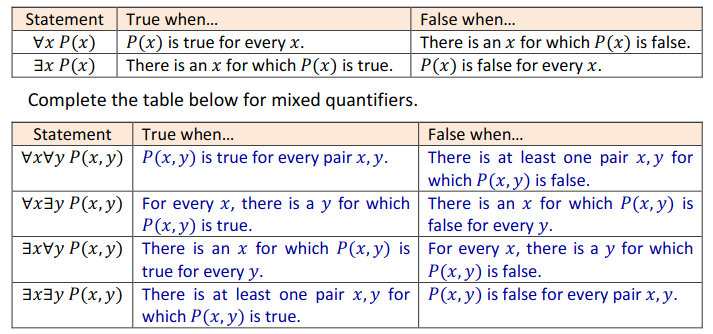
\includegraphics[width = \textwidth]{ttb.png}
\end{frame}

\begin{frame}[fragile]{Question D4}
(to be discussed if there is time)
\end{frame}

\begin{frame}[fragile]{Question 1}
\begin{align*}
Statement: \ &\forall n \in \mathbb{Z}((6\mid n) \rightarrow (2\mid n) \land (3 \mid n) ). &(True) \\
Converse: \ &\forall n \in \mathbb{Z}((2\mid n) \ \land \ (3\mid n) \ \rightarrow (6\mid n) ). &(True) \\
Inverse: \ &\forall n \in \mathbb{Z}(6\nmid n \rightarrow (2\nmid n) \lor (3\nmid n) ). &(True) \\
Contrapositive: \ &\forall n \in \mathbb{Z}((2\nmid n) \lor (3\nmid n) \rightarrow (6\nmid n) ). &(True)
\end{align*} 
\end{frame}

\begin{frame}[fragile]{Question 1}
\begin{align*}
Statement: \ &\forall r \in \mathbb{R}(r>3 \rightarrow r^2>9). &(True) \\
Converse: \ &\forall r \in \mathbb{R}(r^2>9 \rightarrow r>3). &(False) \\
Inverse: \ &\forall r \in \mathbb{R}(r\leq 3 \rightarrow r^2\leq 9).  &(False) \\
Contrapositive: \ &\forall r \in \mathbb{R}(r^2\leq 9 \rightarrow r\leq 3). &(True)
\end{align*} 
Counterexample for converse and inverse statements: Let $r = -5$
\end{frame}

\begin{frame}[fragile]{Question 1}
\begin{align*}
Statement: \ &\forall p, q\text{ that are statements, } ((p  \rightarrow q) \rightarrow \ \sim p ). &(False) \\
Converse: \ &\forall p, q\text{ that are statements, } (\sim p  \rightarrow (p  \rightarrow q)). &(True) \\
Inverse: \ &\forall p, q\text{ that are statements, } (\sim(p  \rightarrow q) \rightarrow p ). &(True) \\
Contrapositive:  \ &\forall p, q\text{ that are statements, } (p  \rightarrow \ \sim(p  \rightarrow q)). &(False)
\end{align*} 
Counterexample for original statement and contrapositive: Let both $p$ and $q$ be true.
\end{frame}

\begin{frame}[fragile]{Question 2}
a) $\forall p \exists q \Big((p \neq q) \land Loves(p, q)\Big)$ \\
b) $Loves(John, Mary) \land \forall x \Big((x \neq John) \rightarrow \ \sim Loves(x, Mary)\Big)$
\end{frame}

\begin{frame}[fragile]{Question 3}
\textbf{Proof}\\
1.Take any integers $a, b, c$.\\
2.Suppose $a-b$ is even and $a- c$ is even. \\
\quad  2.1 There is an integer $s$ s.t. $a - b = 2s$ (defn of even numbers). \\
\quad  2.2 Similarly, there is an integer $t$ s.t. $a-c = 2t$ \\
\quad  2.3 Then $b - c = (a - c) - (a - b) = 2t - 2s = 2 (t-s)$\\
3.Therefore, $b-c$ is even (by definition of even numbers).\\
\end{frame}

\begin{frame}[fragile]{Question 4}
a) Invalid, inverse error \\
b) Valid, universal modus ponens \\
c) Invalid, converse error \\
\end{frame}

\begin{frame}[fragile]{Question 5}
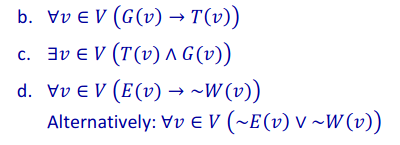
\includegraphics[width=\textwidth]{5bcd.png}
\end{frame}

\begin{frame}[fragile]{Question 5}
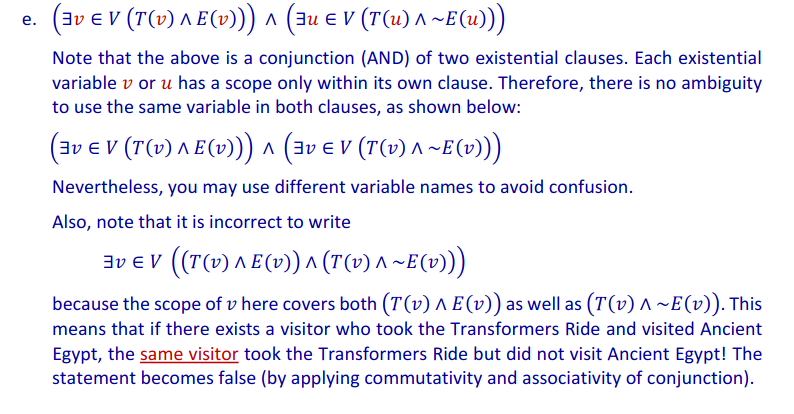
\includegraphics[width=\textwidth]{5e.png}
\end{frame}

\begin{frame}[fragile]{Question 6}
a) False, none of the titles is read by all three female readers \\
b) False, Mr. Dueet doesn't read any Fantasy title \\
c) True, Mr. Dueet reads all the Mystery titles \\
d) True, none of the Fantasy titles is read by Dueet (and Fandi)
\end{frame}

\begin{frame}[fragile]{Question 7}
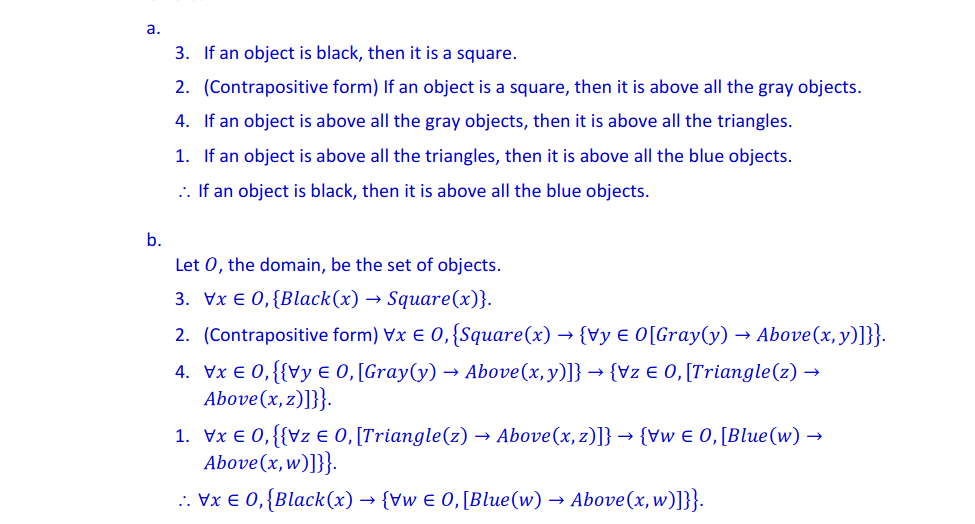
\includegraphics[width=\textwidth]{7.png}
\end{frame}

\begin{frame}[fragile]{Question 8}
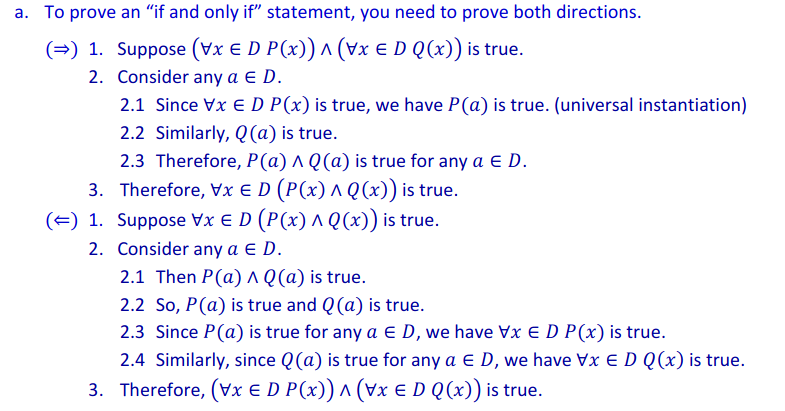
\includegraphics[width=\textwidth]{8a.png}
\end{frame}

\begin{frame}[fragile]{Question 8}
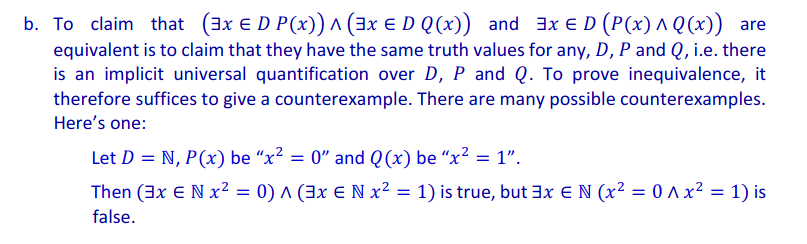
\includegraphics[width=\textwidth]{8b.png}
\end{frame}

\begin{frame}[fragile]{Question 9}
a) $\sim \Big(\forall x, y, \in \mathbb{R} ( x > y \rightarrow x^2 > y ^ 2) \Big) \equiv \exists x, y \in \mathbb{R} (x > y \land x^2 \leq y^2)$ which is true: one example is $(x=1, y = -2)$, so the original statement is false \\
\bigskip
b) Irrelevant counterexample; it does not satisfy the hypothesis ($x > y$)
\end{frame}

\end{document}
